\documentclass[12pt, a4paper]{report}

\usepackage{fontspec}
\setmainfont{Times New Roman}
\setmonofont{Consolas}

\usepackage{polyglossia}
\setmainlanguage{bulgarian}

\usepackage{setspace}
\usepackage{geometry}
\usepackage{listings}
\usepackage{xcolor}
\usepackage{fancyhdr}
\usepackage{graphicx}
\usepackage{hyperref}

\setstretch{1.333}
\geometry{left=30mm, right=20mm, top=25mm, bottom=25mm}

\fancypagestyle{plain}{
  \fancyhf{}
  \fancyfoot[R]{\thepage}
  \renewcommand{\headrulewidth}{0pt}
}
\pagestyle{plain}

% Обединени и коригирани настройки за кода
\definecolor{codegreen}{rgb}{0,0.6,0}
\definecolor{codegray}{rgb}{0.5,0.5,0.5}
\definecolor{codepurple}{rgb}{0.58,0,0.82}
\definecolor{backcolour}{rgb}{0.95,0.95,0.92}

\lstset{
  language=C++,
  backgroundcolor=\color{backcolour},
  commentstyle=\color{codegreen},
  keywordstyle=\color{blue}, % Без \bfseries заради мака
  numberstyle=\tiny\color{codegray},
  stringstyle=\color{codepurple},
  basicstyle=\ttfamily\small\setstretch{1.333}, % С междуредие 16pt
  breakatwhitespace=false,
  breaklines=true,
  captionpos=b,
  keepspaces=true,
  numbers=left,
  numbersep=5pt,
  showspaces=false,
  showstringspaces=false,
  showtabs=false,
  tabsize=4,
  frame=single,
  rulecolor=\color{black!30}
}

\begin{document}
\hfuzz=10pt

\pagenumbering{gobble}
\begin{center}
  
\includegraphics[width=3.5cm]{images/su_logo.jpg}\\[0.8cm]

  \large\bfseries Софийски университет „Св. Климент Охридски“\\[0.3cm]
  \large\bfseries Факултет по математика и информатика\\[2cm]

  \Large КУРСОВ ПРОЕКТ\\
  \large по Обектно-ориентирано програмиране\\[1.5cm]

  \huge\bfseries Приложение за работа с електронни таблици\\[3cm]
\end{center}

\vspace{3cm}
\begin{flushleft}
  Изготвил: \textbf{Антон Вачков} \\
  Специалност: \textbf{Компютърни науки} \\
\end{flushleft}

\newpage
\pagenumbering{arabic}
\tableofcontents
\newpage

\chapter{Увод}

\section{Описание и идея на проекта}
Основната идея на проекта е създаването на конзолно приложение на езика \textit{C++} за управление на електронни таблици. Програмата предоставя текстов интерфейс, чрез който потребителят може да зарежда данни от файл в паметта, да редактира съдържанието на отделните клетки и да визуализира таблицата. Поддържа се работа с различни типове данни в една и съща таблица, както и динамично изчисляване на математически формули с препратки към други клетки. Всички промени се запазват обратно в текстов файл при изрично желание на потребителя.

Проектът е с отворен код и достъпен в GitHub на адрес: \\ \url{https://github.com/AVachkov/Spreadsheet}.

\section{Цел и задачи на разработката}

Целта на проекта е да се изгради работеща система, която абстрахира сложността на вътрешното представяне на данните и се фокусира изцяло върху същността на тяхната обработка, изчисляване и сигурно съхранение.

Основните задачи, решени по време на разработката, са:

\begin{itemize}
  \item \textbf{Структура на данните:} Създаване на общ базов клас и отделни класове за поддържаните хетерогенни типове съдържание: цели числа, дробни числа, символни низове и формули.
  \item \textbf{Взаимодействие между класовете:} Правилно организиране на връзките и комуникацията между главния клас на таблицата и отделните обекти за клетките, за да работят заедно като единна система.
  \item \textbf{Пресмятане на формули:} Реализиране на алгоритъм, който чете математически изрази, поддържа основните аритметични операции (\texttt{+}, \texttt{-}, \texttt{*}, \texttt{/}, \texttt{\^{}}), спазва техния приоритет и преобразува типовете при нужда (например празни клетки и нечислови низове се оценяват като 0).
  \item \textbf{Изчисляване на препратките:} Извличане на стойности от конкретни адреси (например \texttt{R1C1}), като при грешка във формулата или деление на нула програмата не прекъсва своето изпълнение, а просто извежда \texttt{"ERROR"} в съответната клетка.
  \item \textbf{Защита от зацикляне:} Справяне с проблема, при който две клетки зависят една от друга, за да се предотврати блокиране на програмата.
  \item \textbf{Управление на паметта:} Внимателно и оптимално заделяне и освобождаване на динамична памет, за да няма утечки (\textit{memory leak}).
  \item \textbf{Работа с файлове:} Реализиране на команди за зареждане (\texttt{open}) и записване (\texttt{save}, \texttt{saveas}) на таблицата.
\end{itemize}

\section{Структура на документацията}
Настоящата документация е организирана в пет основни глави:
\begin{itemize}
  \item \textbf{Глава 1 - Увод:} Описва идеята на проекта, целите и основните решени задачи.
  \item \textbf{Глава 2 - Преглед на предметната област:} Разглежда дефинициите за типовете данни, формулите и функционалните изисквания.
  \item \textbf{Глава 3 - Проектиране:} Представя архитектурата на приложението и ООП дизайна.
  \item \textbf{Глава 4 - Реализация и тестване:} Описва детайли по управлението на паметта, алгоритмите и проведените тестове.
  \item \textbf{Глава 5 - Заключение:} Обобщава постигнатите резултати и дава насоки за бъдещо развитие.
\end{itemize}
\chapter{Преглед на предметната област}

\section{Основни дефиниции, концепции и алгоритми}
Електронната таблица се моделира като правоъгълна матрица в оперативната памет. Основните градивни единици са клетките, които могат да бъдат празни или да съдържат: числа, текст (в кавички) или формули (започващи с \texttt{=}). За пресмятане на формулите и извличане на стойности от други клетки се използва рекурсивен алгоритъм.

\section{Проблеми и сложност}
Основно предизвикателство е как формулите с препратки да извличат нужните стойности, без да се създава силна зависимост към цялостната структура на таблицата.

Друг съществен проблем възниква при зареждането на данните. Динамичното изчисляване на формули не може да се извършва линейно по време на четенето от файл, тъй като те могат да реферират към клетки, които все още не са заредени в паметта.

\section{Методи за решаване на проблемите}
За справяне с дефинираните алгоритмични предизвикателства са приложени следните подходи:

\begin{itemize}
  \item \textbf{Взаимодействие и достъп до данни:} За да се избегне подаването на директен достъп до целия масив с данни, се използва механизъм за индиректно извличане на стойности. По този начин формулите получават нужните данни в реално време, без да се нарушава капсулацията на таблицата.

  \item \textbf{Отложено изчисляване на формули:} Първо цялата таблица се зарежда напълно в паметта, а след това за извличане на липсващи стойности от реферирани клетки се използва рекурсия. За да се предотврати безкраен цикъл при взаимнозависими клетки (циклични препратки), преди всяко извикване временно се задава статус на активно изчисляване. При повторно засичане на такъв статус, алгоритъмът разпознава зациклянето и безопасно прекъсва операцията.
\end{itemize}

\section{Потребителски и качествени изисквания}

\textbf{Функционални изисквания (Потребителски):}
Приложението предоставя конзолен интерфейс (CLI). Таблиците се зареждат от текстов файл (стойности, разделени със запетаи). Потребителят разполага със следните команди:
\begin{itemize}
  \item Файлови: \texttt{open <file>}, \texttt{close}, \texttt{save}, \texttt{saveas <file>}, \texttt{help}, \texttt{exit}.
  \item Операционни: \texttt{edit <address> <value>} (промяна на клетка) и \texttt{print} (отпечатване с автоматично подравняване).
\end{itemize}

\textbf{Качествени изисквания (Нефункционални):}
Системата трябва да осигурява висока стабилност при невалидни данни – да конвертира празни и текстови клетки до 0 при изчисление, и да индикира грешки (напр. деление на нула) без срив на програмата. Приложението трябва да е устойчиво на неточно въвеждане, като автоматично игнорира излишни интервали около разделителите.
\chapter{Проектиране}

\section{Обща архитектура – ООП дизайн}
Архитектурата на приложението е изградена на базата на обектно-ориентираното програмиране, като логиката е разпределена между главния
клас \texttt{Spreadsheet} и йерархията на класа \texttt{Cell}.

\textbf{Клас \texttt{Spreadsheet}:}
Това е главният клас, който капсулира двумерната матрица от указатели към базовия клас \texttt{Cell}. Той не само предоставя публичен
интерфейс за основните команди (зареждане, запис, редактиране, отпечатване), но и изцяло управлява жизнения цикъл на клетките
(динамичната памет). В неговите отговорности влизат още десериализацията на входните данни и стартирането на процеса по разрешаване
на зависимостите във формулите.

\textbf{Йерархия на клетките (\texttt{Cell}):}
Всяка клетка е представена чрез базов клас \texttt{Cell}, който задава общи задължителни виртуални методи (за отпечатване, извличане
на дължина на съдържанието и извличане на числова стойност). За различните видове данни са създадени конкретни класове-наследници:
за цели числа (\texttt{WholeNumberCell}), дробни числа (\texttt{DecimalNumberCell}), текст (\texttt{TextCell}), формули
(\texttt{FormulaCell}), празни клетки (\texttt{EmptyCell}) и грешки (\texttt{ErrorCell}).

\textbf{Изчисляване на формули (\texttt{Formula} и \texttt{FormulaCell}):}
Класът \texttt{FormulaCell} съдържа в себе си обект от тип \texttt{Formula}, който изцяло поема логиката по анализиране и
пресмятане на математически изрази. При проектирането на тази връзка е избегната първоначалната идея за подаване на директен
указател от формулата към таблицата, тъй като това би обвързало класовете твърде силно. Вместо това е внедрено по-елегантно
решение с \texttt{std::function}. Методът \texttt{solveFormula} извършва пресмятанията над отделните компоненти на израза,
като разчита на подадена от \texttt{Spreadsheet} ламбда функция за индиректно извличане на стойности в реално време. По този
начин \texttt{Formula} остава напълно капсулиран, изолиран от вътрешната структура на матрицата и независим от нейната организация.

\section{Диаграми и извадки от кода}

\subsection*{Диаграма на класовете}
Структурата на класовете и полиморфните връзки между главния мениджър \texttt{Spreadsheet}, базовия абстрактен клас \texttt{Cell} и неговите конкретни наследници са представени на фиг. \ref{fig:class_diagram}.

\begin{figure}[h]
  \centering
  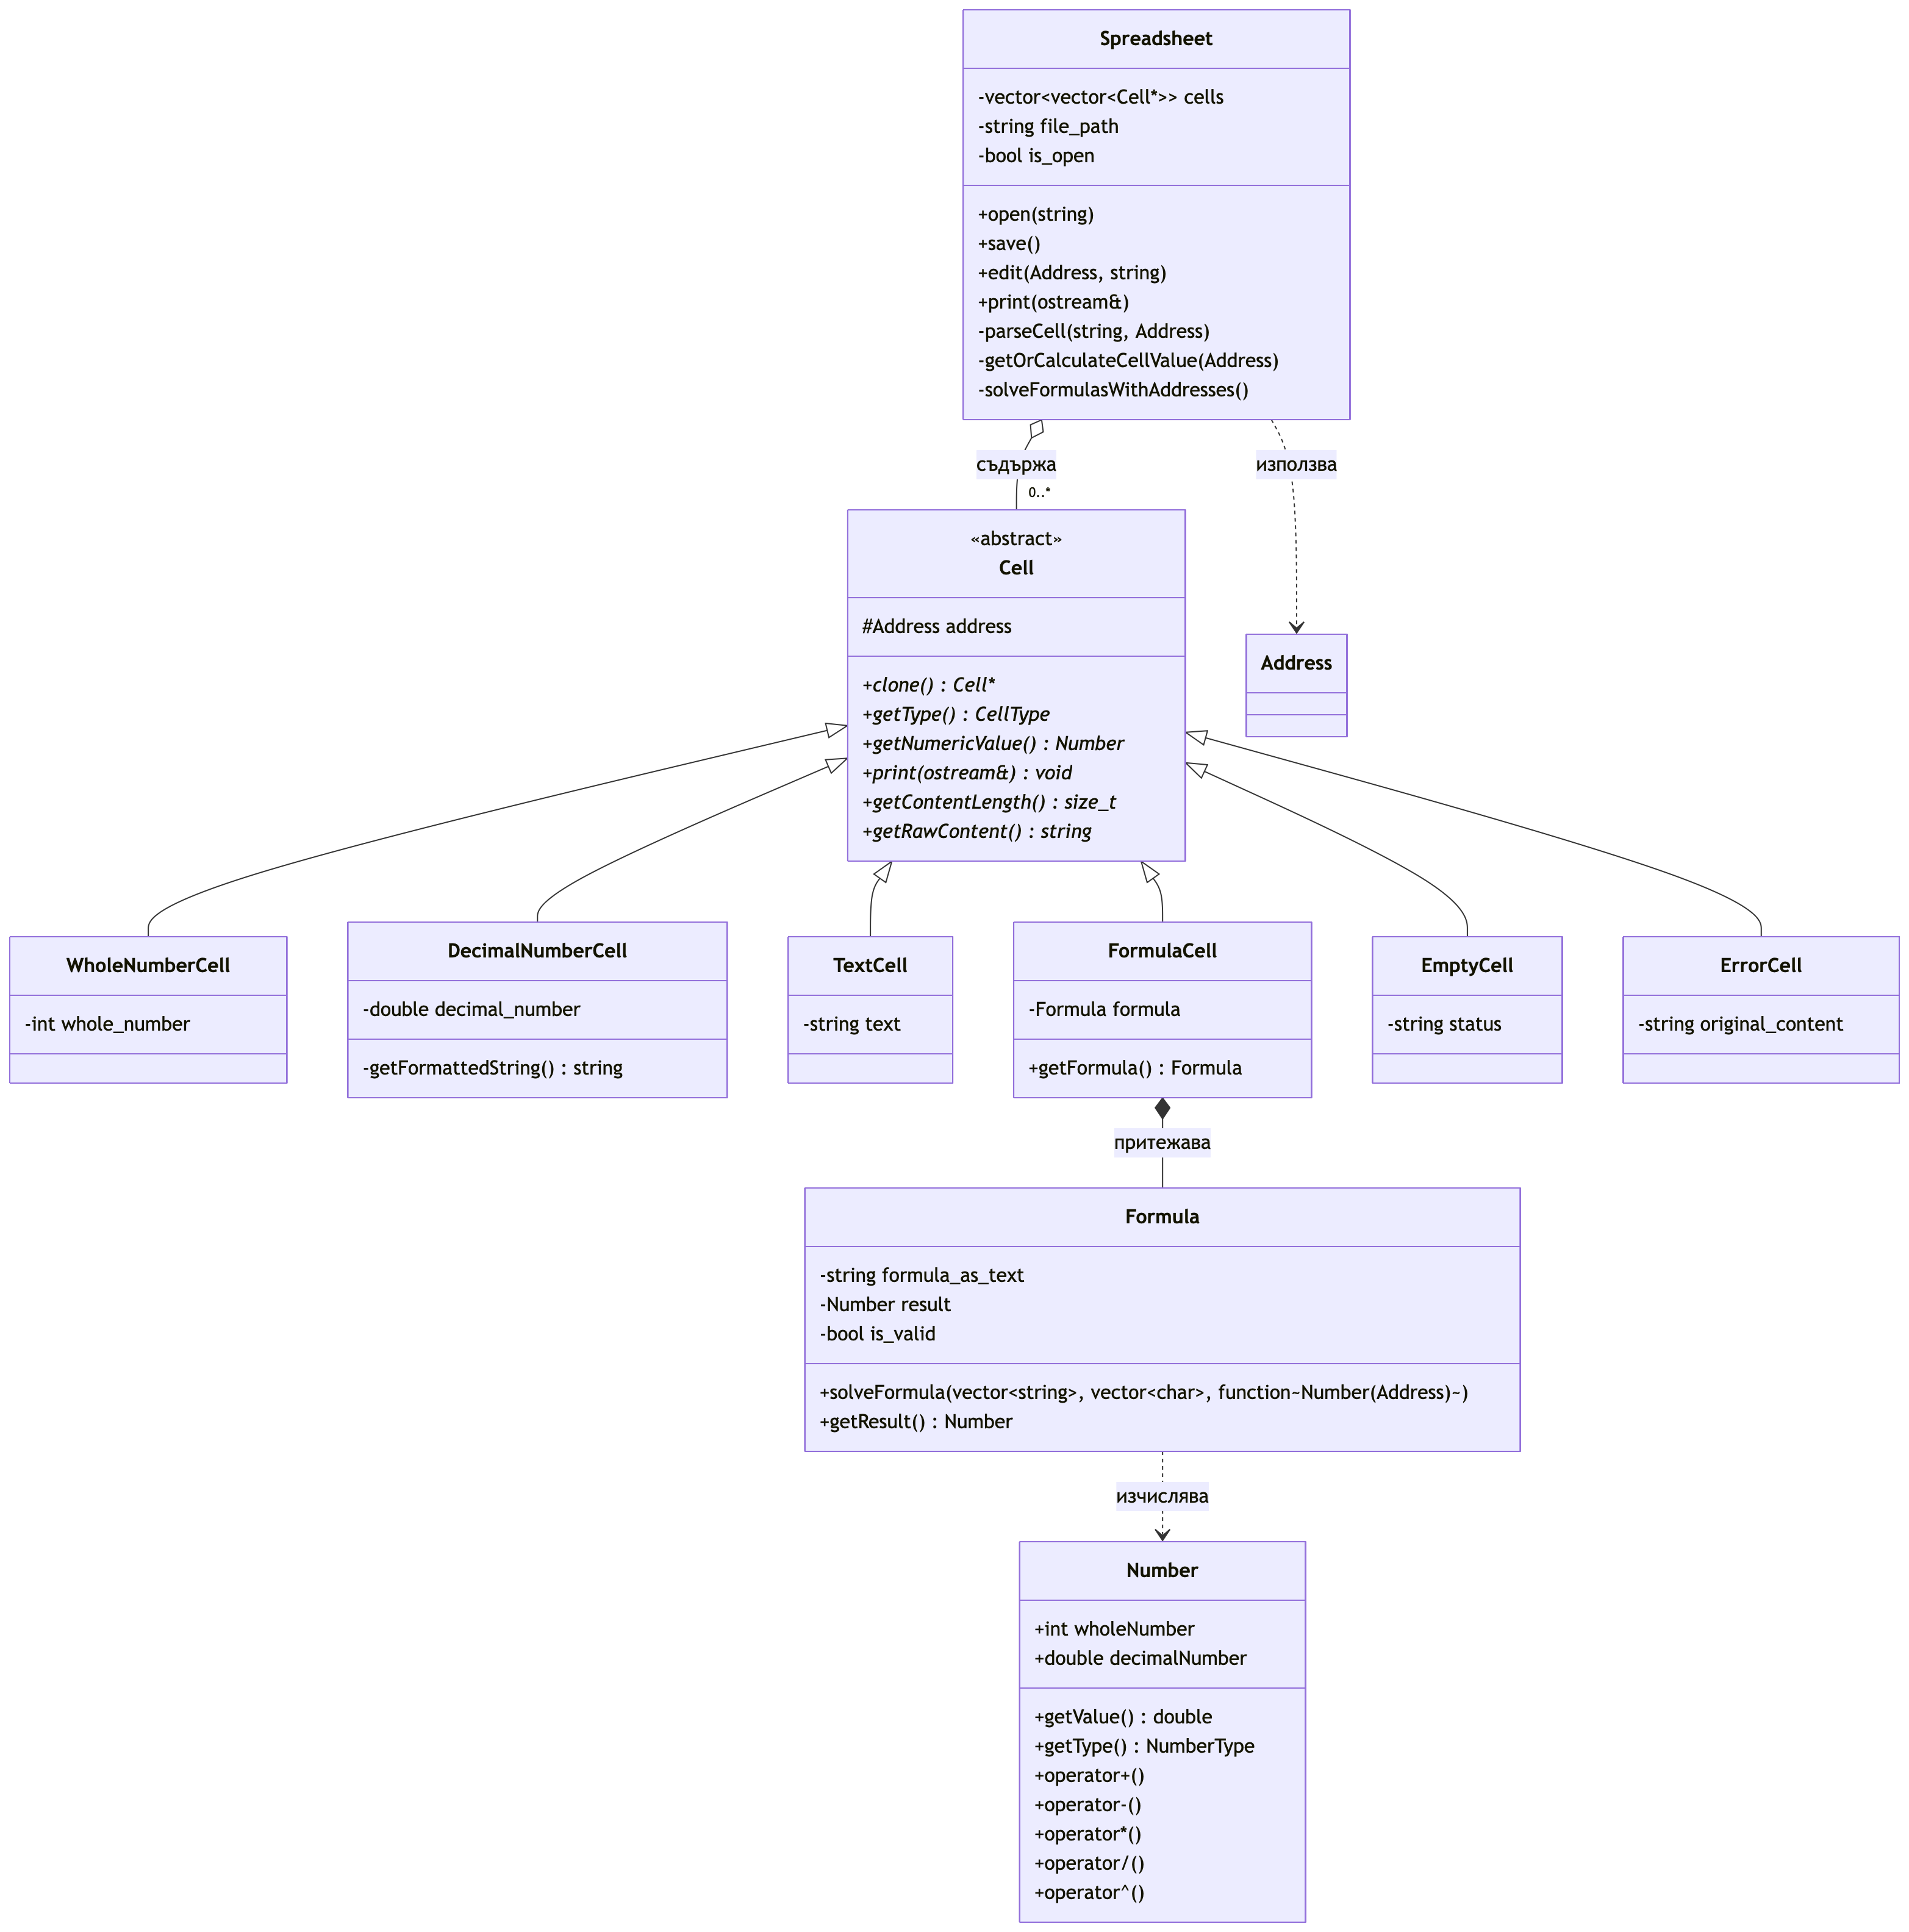
\includegraphics[width=0.9\textwidth]{images/class_diagram.png}
  \caption{Структурна диаграма на класовете}
  \label{fig:class_diagram}
\end{figure}

\subsection*{Поведенчески модел: Индиректно извличане на стойности}
Следната извадка от метода \texttt{getOrCalculateCellValue} демонстрира ключовия поведенчески модел – как \texttt{Spreadsheet} обработва формулите и им подава ламбда функция, улавяйки указателя \texttt{this}. Това позволява на обекта \texttt{Formula} да извлича стойности от други клетки в реално време. Преди извикването, клетката временно получава статус \texttt{"CALCULATING"}, за да се предотврати безкрайна рекурсия:

\begin{lstlisting}[language=C++]
std::vector<std::string> tokens;
std::vector<char> operators;

std::string formulaText = formula.getFormulaText();
tokenize(formulaText, tokens, operators);

// Временно заместване за защита от циклични препратки
delete cells[a.row - 1][a.col - 1];
cells[a.row - 1][a.col - 1] = new EmptyCell(a, "CALCULATING");

try
{
    // Подаване на ламбда функция, чрез която формулата
    // получава възможност индиректно и рекурсивно да
    // извлича непресметнати стойности
    formula.solveFormula(tokens, operators,
        [this](Address a) {
            return this->getOrCalculateCellValue(a);
        });

}
catch (const std::runtime_error &e)
{
    delete cells[a.row - 1][a.col - 1];
    cells[a.row - 1][a.col - 1] = new ErrorCell(a, formulaText);
    throw;
}
\end{lstlisting}
\chapter{Реализация и тестване}

\section{Реализация на класове}
В основата на реализацията на електронната таблица стои полиморфният контейнер (правоъгълна матрица от клетки), управляван от класа \texttt{Spreadsheet}. Тъй като таблицата трябва да съхранява хетерогенни данни (текст, числа и формули) в обща структура, тя е реализирана като двумерен вектор от указатели към базовия абстрактен клас \texttt{Cell}:

\begin{lstlisting}[language=C++]
// Декларация на основния контейнер в класа Spreadsheet
std::vector<std::vector<Cell *>> cells;
\end{lstlisting}

Използването на указатели към базовия клас позволява прилагането на полиморфизъм. Когато \texttt{Spreadsheet} изпълнява команди като отпечатване или изчисляване, той извиква виртуалните методи (като \texttt{print()} или \texttt{getNumericValue()}) директно през общия интерфейс на \texttt{Cell}. По този начин главният клас управлява всички видове клетки по абсолютно еднакъв начин, без нуждата да проверява ръчно дали конкретният обект зад указателя е число, текст или формула.

За да се попълни тази матрица с реални обекти при десериализация или редактиране, е имплементиран частният метод \texttt{parseCell}. Тъй като останалата част от логиката работи само с абстрактни указатели, този метод служи като мост – той директно приема текстовия низ, разпознава типа му чрез помощни функции и заделя памет за съответния наследник:

\begin{lstlisting}[language=C++]
// Метод за разпознаване и създаване
// на конкретни обекти клетки
Cell* parseCell(const std::string &token, Address a);
\end{lstlisting}

По този начин процесът по разпознаване на типовете е капсулиран на едно единствено място в кода, което улеснява бъдещото добавяне на нови видове клетки.

\subsection*{Реализация на връзката между таблицата и формулите}
Едно от основните имплементационни предизвикателства е взаимодействието между класа \texttt{Spreadsheet} и обектите от тип \texttt{Formula}. Първоначалната идея за осигуряване на достъп на формулите до клетките беше подаване на директен указател към таблицата, за да се предотврати копирането на целия двумерен вектор. Тъй като обаче формулите нямат реална нужда от достъп до всички клетки, бе реализирано по-елегантно решение чрез \texttt{std::function}.

Основният механизъм, който прави това възможно, е т.нар. \textit{capture list} (списък за улавяне) в C++. Чрез него ламбда изразът в \texttt{solveFormula} „улавя“ указателя към текущата инстанция на таблицата (\texttt{[this]}) и го предава индиректно:

\begin{lstlisting}[language=C++]
// Ламбда функция за индиректно извличане на стойности
formula.solveFormula(tokens, operators, [this](Address a) {
    return this->getOrCalculateCellValue(a);
});
\end{lstlisting}

По този начин обектът \texttt{Formula} извлича стойности от адреси в реално време, без изобщо да се интересува от структурата на двумерния масив и без да нарушава капсулацията на \texttt{Spreadsheet}.

\subsection*{Използван външен код}
Логиката във функцията \texttt{TextCell::getContentLength()} във файла \texttt{cell.cpp} е взета от генеративен модел, тъй като стандартният метод \texttt{std::string::length()} не работи коректно за текст на кирилица.

\section{Управление на паметта, алгоритми и оптимизации}

\textbf{Управление на ресурсите чрез „Голямата четворка“} \\
Тъй като \texttt{Spreadsheet} управлява вектор от указатели към динамично заделена памет, в него е реализирана „Голямата четворка“ (\textit{Big Four}) -- дефинирани са конструктор по подразбиране, копиращ конструктор, оператор за присвояване и деструктор. За нуждите на копирането се използва виртуалният метод \texttt{clone()} от \texttt{Cell}. Всеки наследник връща свое дълбоко копие (\textit{deep copy}), което елиминира риска от споделена памет и предпазва от „двойно освобождаване“ (\textit{double-free}).

\textbf{Полиморфно разрушаване на обекти} \\
Задължителен елемент от йерархията е дефинирането на виртуален деструктор в базовия клас \texttt{Cell}. Той гарантира, че при разрушаване на клетка през указател от базов тип, правилно ще се извърши полиморфно извикване на деструктора на конкретния наследник, предотвратявайки изтичане на памет (\textit{memory leak}).

\textbf{Изчисляване на формули и защита от безкрайна рекурсия} \\
Изчисляването на формули с препратки към други клетки изисква таблицата да бъде предварително заредена в паметта, тъй като даден израз може да реферира към клетка, която все още не е пресметната. Поради този факт стандартното линейно изчисляване по време на самото четене е неприложимо. Процесът е разделен на два етапа: първо се зареждат всички независими клетки (числа, текст и формули без препратки), след което се прилага стратегия за отложено изчисляване -- при срещане на препратка във формула, алгоритъмът се извиква рекурсивно за съответната клетка, за да извлече стойността ѝ в реално време.

За да се предотврати безкрайна рекурсия при циклични зависимости (напр. две клетки, които взаимно се реферират), преди всяко рекурсивно извикване текущата клетка се замества с \texttt{EmptyCell} и се маркира временно със статус \texttt{"CALCULATING"} (това е конкретното предназначение на член-данната \texttt{status} в \texttt{EmptyCell}). При повторен опит за достъп до клетка в това състояние се индикира зацикляне и изпълнението се прекъсва безопасно чрез хвърляне на изключение.

\textbf{Оптимизация на матрицата} \\
При четене от файл редовете често съдържат различен брой клетки, което прави структурата в паметта „назъбена“ (\textit{jagged}). Методът \texttt{alignAllCells} допълва матрицата с празни клетки (\texttt{EmptyCell}) до изравняване на всички редове спрямо най-дългия. Това осигурява правилна правоъгълна структура и елиминира риска от грешки при индексиране извън границите.

\section{Планиране и тестови сценарии}

Коректността на системата е проверена чрез примерната таблица, показана на табл. \ref{tab:test_table}.

\begin{table}[h!]
  \centering
  \begin{tabular}{|c|c|c|c|}
    \hline
    10 & 20 & 30 & 40 \\ \hline
    &    &    &    \\ \hline
    10 &    & 1000 &  \\ \hline
    &    &    &    \\ \hline
    & 10 &    &    \\ \hline
  \end{tabular}
  \caption{Начално състояние на тестовата таблица}
  \label{tab:test_table}
\end{table}

Върху нея през конзолния интерфейс са изпълнени сценарии, покриващи нормалната работа и защитите от грешки:

\begin{itemize}
  \item \textbf{Сценарий 1: Изчисляване на формула с валидни адреси} \\
    \textit{Вход:} \texttt{edit R2C1 =R1C1+R1C2} \\
    \textit{Резултат:} Системата успешно събира стойностите (10 и 20). При отпечатване клетката извежда \texttt{30}.

  \item \textbf{Сценарий 2: Операция с празна клетка} \\
    \textit{Вход:} \texttt{edit R2C2 =R3C1+R3C2} \\
    \textit{Резултат:} Тъй като \texttt{R3C2} е празна (интерпретира се като 0), резултатът от израза се оценява коректно на \texttt{10}.

  \item \textbf{Сценарий 3: Защита от деление на нула} \\
    \textit{Вход:} \texttt{edit R4C1 =R1C4/R2C4} \\
    \textit{Резултат:} Клетката \texttt{R2C4} е празна (0). Математическата валидация улавя делението на нула, предпазва програмата от срив и клетката връща \texttt{ERROR}.

  \item \textbf{Сценарий 4: Защита от циклична зависимост} \\
    \textit{Вход:} \texttt{edit R2C1 =R3C3+R2C1} \\
    \textit{Резултат:} Алгоритъмът засича статус \texttt{"CALCULATING"} заради самореференцията, прекъсва цикъла безопасно.
\end{itemize}
\chapter{Заключение}

\section{Обобщение на изпълнението на началните цели}
Проектът успешно изпълни началните си цели, реализирайки работеща конзолна електронна таблица, която обработва различни типове данни и формули.

\section{Насоки за бъдещо развитие и усъвършенстване}
Основна насока е добавянето на номера на редове и колони при принтиране за по-добра прегледност в конзолата. Следваща ключова стъпка е разработването на графичен потребителски интерфейс (GUI), който да замени изцяло текстовия команден ред.

\renewcommand{\bibname}{Използвана литература}

\begin{thebibliography}{9}
  \addcontentsline{toc}{chapter}{\bibname}
  \raggedright
  \urlstyle{same}

  \bibitem{fmi_problems}
  Георгиев, Калин. \textit{Задачи за самоподготовка по Увод в програмирането, Обектно-ориентирано програмиране, Структури от данни и Функционално програмиране}. Факултет по математика и информатика, Софийски университет „Св. Климент Охридски“, 2026.

  \bibitem{fmi_lectures}
  Георгиев, Калин. \textit{Лекции по Обектно-ориентирано програмиране (lecture-notes)}. GitHub,
  \url{https://github.com/stranxter/lecture-notes/tree/master/notes/02_oop}.

  \bibitem{fmi_lekova}
  Лекова, Мая. \textit{Материали по Обектно-ориентирано програмиране (oop-fmi)}. GitHub,
  \url{https://github.com/MayaLekova/oop-fmi}.

  \bibitem{fmi_practicum}
  Костадинов, Теодор и Александър Мандев. \textit{Материали по Обектно-ориентирано програмиране (Object\_oriented\_programming\_FMI)}. GitHub,
  \url{https://github.com/tkostadinov004/Object_oriented_programming_FMI}.

  \bibitem{cppreference}
  ``C++ Reference.'' \textit{cppreference.com}, \url{https://en.cppreference.com/}.

  \bibitem{cplusplus}
  ``C++ Standard Library.'' \textit{cplusplus.com}, \url{https://cplusplus.com/reference/}.

\end{thebibliography}

\end{document}